\subsection{Disturbance Modelling for MPC}
\label{sec:markov}

The disturbance that was of most interest is the load from consumers on the grid.
The assumption that the load disturbance is modelled as a deterministic process is reasonable. 
The load-cycles on the grid are periodic, and therefore it seems reasonable to suggest a machine could predict what a future demand will be.
Hawaii has a very small change in climate throughout the year - from 20 to 25 degrees Celsius, meaning there is not a large change in load between winter and summer months.

A decision was made that a suitable object to model electrical loads was a Markov Chain - as it takes into account differing patterns in demand.
This object allows for interesting behaviour, for example if the grid is on a path that looks like a weekend demand curve, the Markov Chain will more likely predict demands characteristic of weekends.
The Markov Chain has proved reliable in these situations \cite{power:markovP} which is what allowed this decision.

\textbf{What is a Markov Chain?}
A stochastic model that describes a sequence of state changes, in which the probability of the next state change, depends \emph{only} on the state obtained from the previous change.

\subsubsection{Normalizing Data}

Consumers are becoming more and more dependant on electrical power, in the United States alone, power consumption \emph{per household} was only 10,000 kWh per anum, yet in 2010, power consumption was 11,500 kWh per anum \cite{power:growth}.

To find a way of normalizing the power demand data-set - such that more, old data can be used to build the stochastic matrix, a scaling factor that varies with time must be considered.
The scaling factor used is $\zeta(t^{\prime})$, where $t^{\prime}$ is the days since 1/1/2000.

It was assumed $\zeta$ has form:
\begin{equation}
        \zeta(t^{\prime}) = a t^{\prime} + b
\end{equation}
To find coefficients $a$ and $b$, $\max P$ was plotted for each week, and use a Huber regression.

It was found that $a = 202$, $b = 1.97$.

\subsubsection{Markov Chain Formulation}

To start the formulation, power demand was discretised into a array $F$ of size $N$.

If the demand is known to be $\zeta(t^{\prime}) F(i)$ at time $Tk$, then the probability of demand being $F(j)$ at time $T(k+1)$ is represented by the location in a matrix: $M_{i,j,k}$.
The expectation of demand at time $k+1$ is $\sum^{N}_{j=0} \zeta(t^{\prime}) F(j) M_{i,j,k}$. 

The data is discretised into 10 minute time-slices and form the 3-D stochastic matrix from it.

\begin{figure}[bht]
        \centering
\usetikzlibrary{arrows}
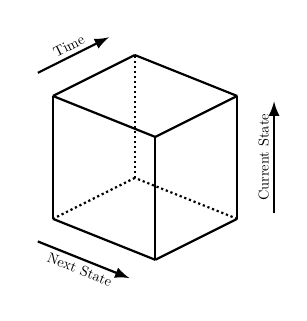
\begin{tikzpicture}[thick,scale=0.52, every node/.style={scale=0.52}]
\coordinate (v1) at (-2,-1.5) {};
\coordinate (v7) at (0,-0.5) {};
\coordinate (v6) at (0.5,-2.5) {};
\coordinate (v5) at (2.5,-1.5) {};
\coordinate (v2) at (-2,-4.5) {};
\coordinate (v3) at (0.5,-5.5) {};
\coordinate (v4) at (2.5,-4.5) {};
\coordinate (v8) at (0,-3.5) {};
\draw  (v1) edge (v2);
\draw  (v2) edge (v3);
\draw  (v3) edge (v4);
\draw  (v5) edge (v4);
\draw  (v6) edge (v5);
\draw  (v1) edge (v6);
\draw  (v1) edge (v7);
\draw  (v7) edge (v5);
\draw  (v6) edge (v3);
\draw [densely dotted] (v4) edge (v8);
\draw [densely dotted] (v8) edge (v2);
\draw [densely dotted] (v8) edge (v7);
\node (v11) at (-2.5,-1) {};
\node (v12) at (-0.5,0) {};
\node (v13) at (-2.5,-5) {};
\node (v14) at (0,-6) {};
\node (v9) at (3.4,-4.5) {};
\node (v10) at (3.4,-1.5) {};\tikzstyle{myedgestyle} = [-latex]
        \draw [-latex] (v11) edge node[sloped, anchor=center, above] {Time} (v12);
        \draw [-latex] (v13) edge node[sloped, anchor=center, below] {Next State} (v14);
        \draw [-latex] (v9) edge node[sloped, anchor=center, above] {Current State} (v10);
\end{tikzpicture}
        \caption{A simplified view of what the stochastic matrix, $M$ will look like.} \label{fig:markov}
\end{figure}
For each day, $k=0$ was set at midnight.
Then to the following for each day of data:

By considering time $k$ (which sets which layer to edit), the $i$ state the system is in is known (which row on the stochastic matrix is being edited).
The state for time $k+1$, which shall be called $i^\prime$ is observed and passed to the next step.
Knowing $i$, $j = i^\prime$, and $k$ - location $M_{i,i^\prime,k}$ is incremented by one.

At this stage a matrix that documents all the state transitions exists - where states were from and where they were to at discrete times.
Only 5 years ($\approx 1800$ days) of data is available, however if the contents of a single row are plotted, Gaussian-like behaviour was observed.
Most probability distributions tend towards the Gaussian for large $n$, this is known as the Central Limit Theorem.

By assuming statistics for state transition is Gaussian in behaviour, it is possible under \emph{Maximum Likelihood Estimation} to estimate centroid location, as well as variance and fit a Gaussian to it.
This hopefully more accurately captures the dynamics of the real system, given the dataset used was not large.

\subsubsection{Obtaining a Disturbance Prediction}

A simple algorithm was developed that takes a walk through the matrix.
The probability of state change is defined by the stochastic matrix, this was used by the algorithm to walk through the data set and generate a predicted load pattern.
By running many (on the order of 10000) runs through the data, the mean path is calculated which is the predicted disturbance.
